\section{Proof of the sharp testing profile}\label{sec:testing}
We use
\[
\TV(P,Q)=\frac12\sum_y|P(y)-Q(y)|,\qquad
\chi^2(P\Vert Q)=\sum_y\frac{(P(y)-Q(y))^2}{Q(y)}
\]
for finite probability measures with $Q>0$. Throughout, empty products equal
$1$, empty sums equal $0$, and the maximum of an empty family of nonnegative
bounds equals $0$. In particular, these conventions include graphs with no
cycles. The factorization proved above implies
\begin{equation}\label{eq:factor}
\frac{dP_G}{dQ_G}(y)=
\prod_{C\in\mathcal C(G)}
\frac{\mu_{|C|,N}(y_C)}{\pi_{|C|,N}(y_C)},\qquad
1+\chi^2(P_G\Vert Q_G)=
\prod_{C\in\mathcal C(G)}(1+v_{|C|,N}).
\end{equation}
Bridges have identical factors in both experiments. Deleting one edge from every
cycle makes the remaining observations exactly independent.

\subsection{A product experiment lemma}
\begin{lemma}[Many small independent likelihood increments]\label{lem:lan}
For each index $n$, let $Q_n=\bigotimes_jQ_{n,j}$ and
$P_n=\bigotimes_jP_{n,j}$ be finite products. Write
\[
\frac{dP_{n,j}}{dQ_{n,j}}=1+u_{n,j},\quad
v_{n,j}=\E_{Q_{n,j}}u_{n,j}^2,\quad
I_n=\sum_jv_{n,j},\quad
\delta_n=\max_j\|u_{n,j}\|_\infty.
\]
Assume $\delta_n\to0$. Then the conclusions of \cref{thm:main} hold with these
$P_n,Q_n,I_n$.
\end{lemma}
\begin{proof}
Each $u_{n,j}$ has mean zero under $Q_{n,j}$. For $|u|\le\delta<1/2$,
Taylor's theorem gives uniform estimates
\[
\log(1+u)=u-\tfrac12u^2+O(\delta u^2),\qquad
|\log(1+u)|\le2|u|.
\]
Consequently, for $Z_n=\sum_j\log(1+u_{n,j})$,
\begin{align*}
\E_{Q_n}Z_n&=-\tfrac12 I_n+O(\delta_n I_n),\\
\Var_{Q_n}Z_n&=I_n+O(\delta_n I_n).
\end{align*}
For the variance estimate, the sum of squared individual means is
$O(\sum_jv_{n,j}^2)\le O(\delta_n^2 I_n)$.
The sum of centered third absolute moments is $O(\delta_n I_n)$.
If $I_n\to\tau\in(0,\infty)$, the Lyapunov central limit theorem gives
\[
Z_n\ \Longrightarrow\ \mathcal N(-\tau/2,\tau)
\quad\text{under }Q_n.
\]
Equivalently one can expand the characteristic functions: the error in the
quadratic approximation is bounded by the same sum of third moments.

Under $P_{n,j}$, expectations satisfy
$\E_{P_{n,j}}f=\E_{Q_{n,j}}(1+u_{n,j})f$.
The same Taylor estimates give mean $v_{n,j}/2+O(\delta_n v_{n,j})$,
variance $v_{n,j}+O(\delta_n v_{n,j})$, and identical third-moment control.
Hence $Z_n\Longrightarrow\mathcal N(\tau/2,\tau)$ under $P_n$.

For total variation use the bounded continuous function
\[
\TV(P_n,Q_n)=\E_{Q_n}(1-e^{Z_n})_+.
\]
If $Z\sim\mathcal N(-\tau/2,\tau)$, direct Gaussian integration gives
\[
\E(1-e^Z)_+
=\Prob(Z<0)-\E(e^Z\one_{\{Z<0\}})
=\Phi(\sqrt\tau/2)-\Phi(-\sqrt\tau/2).
\]
Thus this convergence step does not require a separate
uniform-integrability assumption on likelihood ratios.

If $I_n\to0$, the product identity and Cauchy--Schwarz give
\[
\TV(P_n,Q_n)\le\frac12
\sqrt{\prod_j(1+v_{n,j})-1}
\le\frac12\sqrt{e^{I_n}-1}\longrightarrow0.
\]

If $I_n\to\infty$, use the Hellinger affinity
$A_n=\E_{Q_n}\sqrt{dP_n/dQ_n}$.
For $|u|\le\delta<1$, Taylor's theorem and
$-\frac{d^2}{du^2}\sqrt{1+u}\ge1/(4(1+\delta)^{3/2})$ give
\[
\E_{Q_{n,j}}\sqrt{1+u_{n,j}}
\le1-\frac{v_{n,j}}{8(1+\delta_n)^{3/2}}.
\]
Independence implies
\[
A_n\le\exp\left(-\frac{I_n}{8(1+\delta_n)^{3/2}}\right)\longrightarrow0.
\]
Since $1-\TV(P_n,Q_n)=\sum\min(P_n,Q_n)\le A_n$, the distance tends to one.
Finally the minimum equal-prior average testing error is
$(1-\TV(P_n,Q_n))/2$.
\end{proof}

\subsection{Application and finite bounds}
\begin{proof}[Proof of \cref{thm:main}]
By \cref{thm:cactus}, discard the identical bridge factors, leaving independent
cycle factors. By \cref{thm:distances}, their variances are exactly
\eqref{eq:info}. The cycle lengths form a fixed finite set, so
\cref{cor:paired} gives $\delta_n=O_{q,L}(N^{-1})\to0$.
Apply \cref{lem:lan}.
\end{proof}

For finite parameters, if
$\delta=\max_C\|\mu_{|C|,N}/\pi_{|C|,N}-1\|_\infty<1$ and
$I=\sum_Cv_{|C|,N}$, the proof gives
\begin{equation}\label{eq:finite-bounds}
1-\exp\left(-\frac I{8(1+\delta)^{3/2}}\right)
\le\TV(P_G,Q_G)
\le\min\left\{1,\frac12\sqrt{e^I-1}\right\}.
\end{equation}
The grouped law in \cref{app:groups} computes $I$ and $\delta$ from at most
$\ell+2$ outcomes per cycle.

\begin{corollary}[Relative entropy and testing errors]\label{cor:information}
In \cref{thm:main}, whenever $I_n=O(1)$,
\[
\KL(P_n\Vert Q_n)=\tfrac12 I_n+o(1),\qquad
\KL(Q_n\Vert P_n)=\tfrac12 I_n+o(1).
\]
For sufficiently large $n$ all cycle likelihoods are strictly positive.
If $I_n\to\tau>0$, the likelihood-ratio test has both error probabilities
tending to $\Phi(-\sqrt\tau/2)$.
\end{corollary}
\begin{proof}
Use the two expectations of $Z_n$ in the proof of \cref{lem:lan}.
Strict positivity follows from $\delta_n<1$. The normal limits at threshold
$Z_n=0$ give the two error probabilities.
\end{proof}

\section{Simple optimal statistics and the binary case}\label{sec:statistics}

\subsection{An explicit leading score}
Put $r(\ell)=\lfloor(\ell-1)/2\rfloor$ and define
\[
g_\ell(a)=
\begin{cases}
\prod_i\kappa(a_i),&\ell\text{ odd},\\
K_\ell(a),&\ell\text{ even}.
\end{cases}
\]
For odd cycles this depends only on the number of zero labels.
For even cycles it depends only on that number and, when there are no zeros,
on the resonance bit. These are exactly sufficient statistics because the
likelihood ratio has the same dependence.
Uniformly over the finite label space,
\begin{equation}\label{eq:score-expand}
\frac{\mu_{\ell,N}}{\pi_{\ell,N}}-1
=N^{-r(\ell)}g_\ell+O_{q,\ell}(N^{-r(\ell)-1}).
\end{equation}
Under uniform labels, $g_\ell$ has mean zero and variance
$(q-1)^{2r(\ell)+1}$. For odd $\ell$, factor $\E\kappa^2=q-1$.
For even $\ell$, Parseval counts the $(q-1)^{\ell-1}$ nonzero frequency
vectors satisfying the product constraint.

For a cactus set
\[
T_n=\sum_{C\in\mathcal C_n}N^{-r(|C|)}
\left(g_{|C|}(Y_C)-\E_{\pi_{|C|,N}}g_{|C|}\right).
\]
\begin{proposition}[An asymptotically optimal reduced score]\label{prop:score}
If $I_n\to\tau\in(0,\infty)$ under the hypotheses of \cref{thm:main}, then
\[
\log(dP_n/dQ_n)=T_n-\tfrac12 I_n+o_{Q_n}(1).
\]
The same approximation holds in $P_n$-probability. Hence the test
$T_n>I_n/2$ is asymptotically optimal.
\end{proposition}
\begin{proof}
Let $u_C=\mu/\pi-1$ and $w_C$ be its centered leading term in
\eqref{eq:score-expand}. Then
$\E_{Q_n}(u_C-w_C)=0$ and
$\E_{Q_n}(u_C-w_C)^2=O_{q,L}(N^{-2}v_{|C|,N})$.
Independence yields $\sum_C(u_C-w_C)=o_{Q_n}(1)$.
Also $\sum_Cu_C^2-I_n=o_{Q_n}(1)$, since its variance is bounded by
$\delta_n^2I_n$. The Taylor remainder has expected absolute value
$O(\delta_nI_n)$, and therefore tends to zero.

Under $P_n$, the total mean of the first difference is
$\sum_C\E_Q u_C(u_C-w_C)=O_{q,L}(I_n/N)$ by Cauchy--Schwarz.
Its variance tends to zero by the same estimates and $1+u_C\le1+\delta_n$.
The quadratic sum and Taylor remainder have identical control.
The approximation and continuity of the normal limit give the same errors
as the exact likelihood test.
\end{proof}

\subsection{Over the binary field, cycle parity suffices}
For $q=2$, both scores simplify to
\[
g_\ell(a)=(-1)^{a_1+\cdots+a_\ell}.
\]
For even lengths the single nonzero frequency vector automatically satisfies
the product constraint. Thus the full labelled data can asymptotically be
replaced by one parity bit per cycle, weighted by $N^{-r(\ell)}$.
For cycles of one adjacent pair of lengths, the number of even-parity cycles
is enough after the known centering.

For triangles or squares over $\F_2$, the critical scale is
$m\asymp N^2=2^{4n}$. At $m/N^2\to1$, the limiting distance is
\[
2\Phi(1/2)-1=0.3829249225\ldots,
\]
and the minimum equal-prior error is $0.3085375387\ldots$.
At $m/N^2\to4$, the distance is
$2\Phi(1)-1=0.6826894921\ldots$.
Every tree-shaped subset of the observations remains exactly independent.
These numbers evaluate the proved formula; they are not empirical fits.

\begin{figure}[htbp]
\centering
\IfFileExists{figures/detection_profile.pdf}{
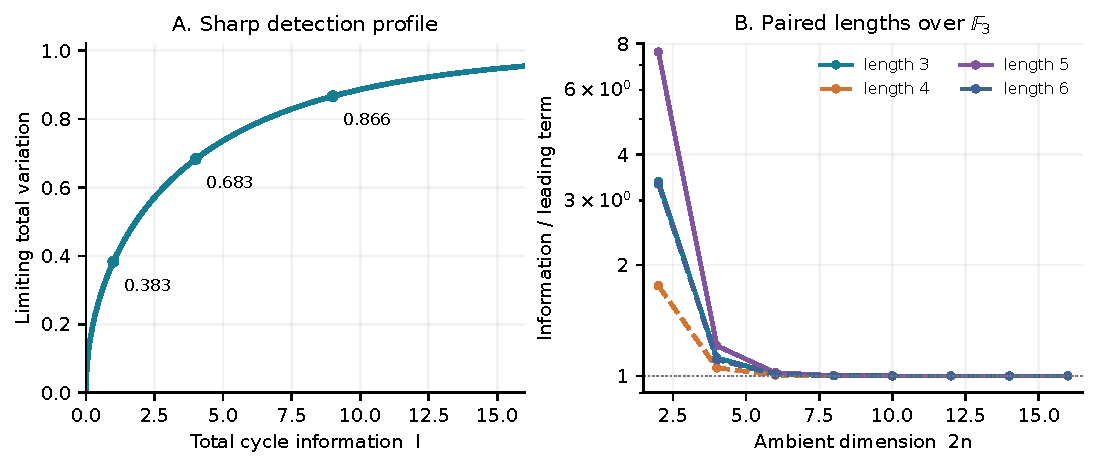
\includegraphics[width=.98\linewidth]{figures/detection_profile.pdf}
}{}
\caption{The sharp detection profile and leading information shared by paired
cycle lengths. The smooth curve is the proved limit. Finite information values
are computed from the exact rational formulas.}
\label{fig:profile}
\end{figure}

